\let\lesson\undefined
\newcommand{\lesson}{\phantomlesson{Bài 7.}}
\section{Bài tập trắc nghiệm}
\begin{enumerate}[label=\bfseries Câu \arabic*:, leftmargin=1.7cm]
	\item \mkstar{1}\\
	Gọi $p$, $V$, $T$ là các thông số trạng thái, $m$ là khối lượng khí, $ M$ là khối lượng mole của khí và $R$ là hằng số khí lí tưởng. Phương trình Clapeyron - Mendeleev có dạng
	\begin{mcq}(4)
		\item $pVT=\dfrac{m}{M}R$.
		\item $\dfrac{pV}{T}=\dfrac{m}{M}R$.
		\item $\dfrac{pV}{T}=\dfrac{M}{m}R$.
		\item $\dfrac{pV}{T}=\dfrac{1}{Mm}R$.
	\end{mcq}
\hideall{
\textbf{Đáp án B.}
}

\item \mkstar{2}\\
Hai phòng kín có thể tích bằng nhau, thông với nhau bằng một cửa mở. Nhiệt độ không khí trong hai phòng khác nhau, thì số phân tử khí trong mỗi phòng so với nhau sẽ 
\begin{mcq}(2)
	\item bằng nhau.
	\item nhiều hơn ở phòng nóng.
	\item nhiều hơn ở phòng lạnh.
	\item phụ thuộc kích thước cửa.
\end{mcq}
\hideall{
\textbf{Đáp án C.}

}

\item \mkstar{2}\\
Cho bốn bình có cùng dung tích và cùng nhiệt độ đựng các khí khác nhau. Khí ở bình nào có áp suất lớn nhất?
\begin{mcq}(2)
	\item Bình 1 đựng $\SI{4}{\gram}$ khí hydrogen.
	\item Bình 2 đựng $\SI{22}{\gram}$ khí carbon dioxide.
	\item Bình 3 đựng $\SI{7}{\gram}$ khí nitrogen.
	\item  Bình 4 đựng $\SI{4}{\gram}$ khí oxygen.
\end{mcq}
\hideall{
\textbf{Đáp án A.}
}

\item \mkstar{2}\\
Một lượng khí hydrogen ở $\SI{27}{\celsius}$ dưới áp suất $\SI{99720}{\pascal}$. Khối lượng riêng của khí là
\begin{mcq}(4)
	\item $\SI{0.08}{\kilogram/\meter^3}$.
	\item $\SI{0.80}{\kilogram/\meter^3}$.
	\item $\SI{0.88}{\kilogram/\meter^3}$.
	\item $\SI{0.068}{\kilogram/\meter^3}$.
\end{mcq}
\hideall{
\textbf{Đáp án A.}\\
$$pV=\dfrac{m}{ M}RT\Rightarrow \rho=\dfrac{m}{V}=\dfrac{p M}{RT}=\SI{0.08}{\kilogram/\meter^3}.$$
}

\item \mkstar{3}\\
Hai bình thuỷ tinh A và B cùng chứa khí helium. Áp suất khí ở bình A gấp đôi áp suất khí ở bình B. Dung tích của bình B gấp đôi bình A. Khi bình A và B cùng nhiệt độ thì
\begin{mcq}
	\item số nguyên tử ở bình A nhiều hơn số nguyên tử ở bình B.
	\item số nguyên tử ở bình B nhiều hơn số nguyên tử ở bình A.
	\item số nguyên tử ở hai bình như nhau.
	\item mật độ nguyên tử ở hai bình như nhau.
\end{mcq}
\hideall{
\textbf{Đáp án C.}
}

\item \mkstar{3}\\
Hai bình chứa khí lí tưởng ở cùng nhiệt độ. Bình B có dung tích gấp đôi bình A, có số phân tử bằng nửa số phân tử trong bình A. Áp suất khí trong bình B so với áp suất khí trong bình A thì
\begin{mcq}(4)
	\item bằng nhau.
	\item bằng một nửa.
	\item bằng $\dfrac{1}{4}$.
	\item gấp đôi.
\end{mcq}
\hideall{
\textbf{Đáp án C.}
}


\item\mkstar{3}\\
Khí cầu có dung tích $\SI{328}{\meter^3}$ được bơm khí hydrogen. Khi bơm xong, hydrogen trong khí cầu có nhiệt độ $\SI{27}{\celsius}$, áp suất $\SI{0.9}{atm}$. Nếu mỗi giây bơm được $\SI{2.5}{\gram}$ khí vào khí cầu thì thời gian để bơm là
\begin{mcq}(4)
	\item $\SI{2}{\hour}$.
	\item $\SI{160}{\minute}$.
	\item $\SI{960}{\second}$.
	\item $\SI{1.5}{\hour}$.
\end{mcq}
\hideall{
\textbf{Đáp án B.}\\
}

\item \mkstar{3}\\
Bình chứa được $\SI{7}{\gram}$ khí nitrogen ở nhiệt độ $\SI{27}{\celsius}$ dưới áp suất $\SI{5.11E5}{\pascal}$. Người ta thay khí nitrogen bằng khí X. Lúc này nhiệt độ khí X trong bình là $\SI{53}{\celsius}$, bình chỉ chứa được $\SI{4}{\gram}$ khí đó ở áp suất $\SI{44.4e5}{\pascal}$. Khí X là 
\begin{mcq}(4)
	\item $\ce{H_2}$.
	\item $\ce{He}$.
	\item $\ce{O_2}$.
	\item $\ce{CO_2}$.
\end{mcq}
\hideall{
\textbf{Đáp án A.}
}

\item \mkstar{3}\\
Trong một ống dẫn khí tiết diện đều $S=\SI{5}{\centi\meter^2}$ có khí $\ce{CO_2}$ chảy qua ở nhiệt độ $\SI{35}{\celsius}$ và áp suất $\SI{3E5}{\pascal}$. Trong thời gian $\SI{10}{\minute}$ có $m=\SI{3}{\kilogram}$ khí $\ce{CO_2}$ qua ống. Tốc độ của dòng khí là
\begin{mcq}(4)
	\item $\SI{2.085}{\meter/\second}$.
	\item $\SI{2.065}{\meter/\second}$.
	\item $\SI{1.94}{\meter/\second}$.
	\item $\SI{1.616}{\meter/\second}$.
\end{mcq}
\hideall{
\textbf{Đáp án C.}\\
Thể tích khí:
$$V=\dfrac{mRT}{ M p}\approx\SI{0.582}{\meter^3}.$$
Tốc độ dòng khí:
$$v=\dfrac{V}{St}=\SI{1.94}{\meter/\second}.$$
}

\item \mkstar{3}\\
Một khối khí lí tưởng được chứa trong bình kín ở nhiệt độ $\SI{300}{\kelvin}$ và áp suất $\SI{40}{atm}$. Cho một nửa lượng khí thoát ra khỏi bình thì áp suất còn $\SI{19}{atm}$. Nhiệt độ của khối khí lúc này là
\begin{mcq}(4)
	\item $\SI{10}{\celsius}$.
	\item $\SI{22}{\celsius}$.
	\item $\SI{15}{\celsius}$.
	\item $\SI{12}{\celsius}$.
\end{mcq}
\hideall{
\textbf{Đáp án D.}\\
\begin{center}
		\begin{tabular}{C{4cm} C{3cm} C{4cm}}
			\colorbox{yellow}{\textcolor{red}{\textbf{Trạng thái 1}}} & $\xrightarrow[V=\text{const} ]{ n_2= n_{1}/2}$ & \colorbox{yellow}{\textcolor{red}{\textbf{Trạng thái 2}}}\\
			$p_1=\SI{40}{atm}$ & &$p_2=\SI{19}{atm}$\\
			$T_1=\SI{300}{\kelvin}$ & & $T_2=?$
		\end{tabular}
	\end{center}
$$\dfrac{p_1}{p_2}=\dfrac{ n_1}{ n_2}\cdot\dfrac{T_1}{T_2}\Rightarrow T_2=\SI{285}{\kelvin}\Rightarrow t_2=\SI{12}{\celsius}.$$
}

\item \mkstar{3}\\
Một lượng khí hydrogen trong bình ở áp suất $\SI{3}{atm}$, nhiệt độ $\SI{27}{\celsius}$. Đun nóng khí đến $\SI{127}{\celsius}$. Do bình hở nên $3/4$ lượng khí thoát ra ngoài. Áp suất khí trong bình bây giờ là
\begin{mcq}(4)
	\item $\SI{2}{atm}$.
	\item $\SI{0.75}{atm}$.
	\item $\SI{1}{atm}$.
	\item $\SI{4}{atm}$.
\end{mcq}
\hideall{
\textbf{Đáp án C.}\\
\begin{center}
	\begin{tabular}{C{4cm} C{3cm} C{4cm}}
		\colorbox{yellow}{\textcolor{red}{\textbf{Trạng thái 1}}} & $\xrightarrow[V=\text{const} ]{ n_2= n_{1}/4}$ & \colorbox{yellow}{\textcolor{red}{\textbf{Trạng thái 2}}}\\
		$p_1=\SI{3}{atm}$ & &$p_2=?$\\
		$T_1=\SI{300}{\kelvin}$ & & $T_2=\SI{400}{\kelvin}$
	\end{tabular}
\end{center}
$$\dfrac{p_2}{p_1}=\dfrac{ n_2}{ n_2}\cdot\dfrac{T_2}{T_1}\Rightarrow p_2=\SI{1}{atm}.$$
}

\item \mkstar{3}\\
Một bình chứa $\SI{1}{\kilogram}$ khí ở áp suất $\SI{E6}{\pascal}$. Người ta lấy ở bình ra một lượng khí cho tới khi áp suất của khí trong bình còn lại $\SI{4E5}{\pascal}$. Coi nhiệt độ của khối khí không đổi. Lượng khí đã lấy ra là
\begin{mcq}(4)
	\item $\SI{0.2}{\kilogram}$.
	\item $\SI{0.4}{\kilogram}$.
	\item $\SI{0.8}{\kilogram}$.
	\item $\SI{0.6}{\kilogram}$.
\end{mcq}
\hideall{
\textbf{Đáp án D.}\\
$$pV=\dfrac{m}{ M}RT\Rightarrow \dfrac{p_2}{p_1}=\dfrac{m_2}{m_1}\Rightarrow m_2=\SI{0.4}{\kilogram}.$$
Lượng khí đã lấy ra:
$$\Delta m=m_1-m_2=\SI{0.6}{\kilogram}.$$
}

\item \mkstar{3}\\
Một bình có dung tích $V=\SI{10}{\liter}$ chứa một lượng khí hydrogen bị nén ở áp suất $p=\SI{50}{atm}$ và nhiệt độ $\SI{7}{\celsius}$. Khi nung nóng bình, do bình hở nên có một phần khí thoát ra; phần khí còn lại có nhiệt độ $\SI{17}{\celsius}$ và vẫn ở áp suất như cũ. Khối lượng khí đã thoát ra là
\begin{mcq}(4)
	\item $\SI{1.502}{\gram}$.
	\item $\SI{2.085}{\gram}$.
	\item $\SI{2.064}{\gram}$.
	\item $\SI{1.616}{\gram}$.
\end{mcq}
\hideall{
\textbf{Đáp án A.}\\
$$\dfrac{pV}{T}=\dfrac{m}{ M} R\Rightarrow m=\dfrac{pV M}{RT}.$$
Khối lượng khí đã thoát ra:
$$\Delta m=\dfrac{pV M}{R}\left(\dfrac{1}{T_1}-\dfrac{1}{T_2}\right)\approx\SI{1.502}{\gram}.$$
}

\item \mkstar{3}\\
Một bình chứa khí oxygen nén ở áp suất $p_1=\SI{15}{\mega\pascal}$ và nhiệt độ $t_1=\SI{37}{\celsius}$ có khối lượng (bình và khí) là $M_1=\SI{50}{\kilogram}$. Dùng khí một thời gian, áp suất khí là $p_2=\SI{5}{\mega\pascal}$ ở nhiệt độ $t_2=\SI{7}{\celsius}$, khối lượng của bình và khí còn lại là $M_2=\SI{49}{\kilogram}$. Khối lượng khí còn lại trong bình và dung tích bình chứa là
\begin{mcq}(4)
	\item $\SI{0.58}{\kilogram}$; $\SI{8.5}{\liter}$.
	\item $\SI{0.85}{\kilogram}$; $\SI{4.8}{\liter}$.
	\item $\SI{5}{\kilogram}$; $\SI{7}{\liter}$.
	\item $\SI{3.7}{\kilogram}$; $\SI{15}{\liter}$.
\end{mcq}
\hideall{
\textbf{Đáp án A.}\\
$pV=\dfrac{m}{ M}RT\Rightarrow m=\dfrac{pV M}{RT}$\\
$\Rightarrow \Delta m=m_1-m_2=M_1-M_2$\\
$\Leftrightarrow \dfrac{p_1V M}{RT_1}-\dfrac{p_2V M}{RT_2}=\left(\SI{50E3}{\gram}-\SI{49E3}{\gram}\right)$\\
$\Rightarrow V=\SI{8.5}{\liter};\quad m_2=\dfrac{p_2V M}{RT_2}\approx\SI{0.58}{\kilogram}.$
}

\item \mkstar{3}\\
Biết rằng mỗi khi lên cao thêm $\SI{10}{\meter}$ thì áp suất khí quyển giảm $\SI{1}{\milli\meter Hg}$ và nhiệt độ trên đỉnh núi là $\SI{2}{\celsius}$. Áp suất khí quyển ở chân núi là $\SI{760}{\milli\meter Hg}$. Khối lượng riêng của không khí ở điều kiện tiêu chuẩn (áp suất $\SI{760}{\milli\meter Hg}$ và nhiệt độ $\SI{0}{\celsius}$) là $\SI{1.29}{\kilogram/\meter^3}$. Khối lượng riêng của không khí ở đỉnh núi Fansipan cao $\SI{3140}{\meter}$ là
\begin{mcq}(4)
	\item $\SI{0.85}{\kilogram/\meter^3}$.
	\item $\SI{0.48}{\kilogram/\meter^3}$.
	\item $\SI{0.75}{\kilogram/\meter^3}$.
	\item $\SI{0.96}{\kilogram/\meter^3}$.
\end{mcq}
\hideall{
\textbf{Đáp án C.}\\
\begin{center}
	\begin{tabular}{C{4cm} C{3cm} C{4cm}}
		\colorbox{yellow}{\textcolor{red}{\textbf{Trạng thái 1}}} & $\xrightarrow{ n=\text{const}}$ & \colorbox{yellow}{\textcolor{red}{\textbf{Trạng thái 2}}}\\
		$p_1=\SI{760}{\milli\meter Hg}$ & &$p_2=760-\dfrac{3140}{10}=\SI{446}{\milli\meter Hg}$\\
		$T_1=\SI{273}{\kelvin}$ & & $T_2=\SI{275}{\kelvin}$\\
		$\rho_1=\SI{1.29}{\kilogram/\meter^3}$&&$\rho_2=?$
	\end{tabular}
\end{center}
$$\rho=\dfrac{m}{V}=\dfrac{p M}{RT}.$$
$$\Rightarrow \dfrac{\rho_2}{\rho_1}=\dfrac{p_2}{p_1}\cdot\dfrac{T_1}{T_2}\Rightarrow \rho_2\approx\SI{0.75}{\kilogram/\meter^3}.$$
}

\item \mkstar{3}\\
Một vận động viên leo núi trong mỗi nhịp thở luôn luôn hít vào $\SI{2}{\gram}$ không khí. Biết rằng khối lượng riêng của không khí ở điều kiện tiêu chuẩn (áp suất $\SI{101.3}{\kilo\pascal}$, nhiệt độ $\SI{0}{\celsius}$) là $\SI{1.29}{\kilogram/\meter^3}$. Hỏi khi ở trên núi cao, tại đó không khí có áp suất là $\SI{79.8}{\kilo\pascal}$ và nhiệt độ $\SI{-13}{\celsius}$ thì thể tích không khí mà người ấy hít vào trong mỗi nhịp thở \textbf{gần với giá trị nào nhất} sau đây?
\begin{mcq}(4)
	\item $\SI{1.3}{\liter}$.
	\item $\SI{1.8}{\liter}$.
	\item $\SI{2.5}{\liter}$.
	\item $\SI{1.9}{\liter}$.
\end{mcq}
\hideall{
\textbf{Đáp án D.}\\
\begin{center}
	\begin{tabular}{C{4cm} C{3cm} C{4cm}}
		\colorbox{yellow}{\textcolor{red}{\textbf{Trạng thái 1}}} & $\xrightarrow{ n=\text{const}}$ & \colorbox{yellow}{\textcolor{red}{\textbf{Trạng thái 2}}}\\
		$p_1=\SI{101.3E3}{\pascal}$ & &$p_2=\SI{79.8E3}{\pascal}$\\
		$T_1=\SI{273}{\kelvin}$ & & $T_2=\SI{260}{\kelvin}$\\
		$\rho_1=\SI{1.29}{\kilogram/\meter^3}$&&$\rho_2=?$
	\end{tabular}
\end{center}
$$\rho=\dfrac{m}{V}=\dfrac{p M}{RT}.$$
$$\Rightarrow \dfrac{\rho_2}{\rho_1}=\dfrac{p_2}{p_1}\cdot\dfrac{T_1}{T_2}\Rightarrow \rho_2\approx\SI{1.067}{\kilogram/\meter^3}=\SI{1.067}{\gram/\liter}.$$
Thể tích không khí mà người ấy hít vào trong mỗi nhịp thở khi ở trên núi:
$$V_2=\dfrac{m}{\rho_2}=\SI{1.87}{\liter}.$$
}

\item \mkstar{3}\\
Người ta bơm không khí ở điều kiện tiêu chuẩn vào một bình có thể tích $\SI{5}{\meter^3}$. Sau nửa giờ bình chứa đầy khí ở nhiệt độ $\SI{24}{\celsius}$ và áp suất $\SI{765}{\milli\meter Hg}$. Coi quá trình bơm diễn ra một cách đều đặn. Khối lượng riêng của không khí ở điều kiện tiêu chuẩn là $\rho=\SI{1.29}{\kilogram/\meter^3}$. Khối lượng khí bơm vào trong mỗi giây là
\begin{mcq}(4)
	\item $\SI{7.5}{\gram/\second}$.
	\item $\SI{4.5}{\gram/\second}$.
	\item $\SI{3.3}{\gram/\second}$.
	\item $\SI{5.6}{\gram/\second}$.
\end{mcq}
\hideall{
\textbf{Đáp án C.}\\
\begin{center}
	\begin{tabular}{C{4cm} C{3cm} C{4cm}}
		\colorbox{yellow}{\textcolor{red}{\textbf{Trạng thái 1}}} & $\xrightarrow{ n=\text{const}}$ & \colorbox{yellow}{\textcolor{red}{\textbf{Trạng thái 2}}}\\
		$p_1=\SI{760}{\milli\meter Hg}$ & &$p_2=\SI{765}{\milli\meter Hg}$\\
		$T_1=\SI{273}{\kelvin}$ & & $T_2=\SI{297}{\kelvin}$\\
		$\rho_1=\SI{1.29}{\kilogram/\meter^3}$&&$\rho_2=?$
	\end{tabular}
\end{center}
$$\dfrac{\rho_2}{\rho_1}=\dfrac{p_2}{p_1}\cdot\dfrac{T_1}{T_2}\Rightarrow p_2\approx\SI{1.1936}{\kilogram/\meter^3}=\SI{1.1936}{\gram/\liter}.$$
Khối lượng khí bơm vào mỗi giây
$$\dfrac{m}{t}=\dfrac{V_2\rho_2}{t}\approx\SI{3.3}{\gram/\second}.$$
}

\item \mkstar{3}\\
Cho biết khối lượng riêng của không khí ở điều kiện tiêu chuẩn (nhiệt độ $\SI{273}{\kelvin}$, áp suất $\SI{101.3}{\kilo\pascal}$) là $\SI{1.29}{\kilogram/\meter^3}$. Khối lượng không khí thoát ra khỏi một căn phòng có thể tích $V=\SI{60}{\meter^3}$ khi ta tăng nhiệt độ của phòng từ $T_1=\SI{280}{\kelvin}$ ở áp suất $p_1=\SI{103}{\kilo\pascal}$ đến $T_2=\SI{300}{\kelvin}$ ở áp suất $p_2=\SI{110}{\kilo\pascal}$ là $\Delta m$. Giá trị $\Delta m$ \textbf{gần nhất với giá trị nào} sau đây?
\begin{mcq}(4)
	\item $\SI{0.36}{\kilogram}$.
	\item $\SI{0.29}{\kilogram}$.
	\item $\SI{0.4}{\kilogram}$.
	\item $\SI{0.25}{\kilogram}$.
\end{mcq}
\hideall{
\textbf{Đáp án D.}\\
\begin{center}
	\begin{tabular}{C{3cm} C{2cm} C{3cm} C{2cm} C{3cm}}
		\colorbox{yellow}{\textcolor{red}{\textbf{Trạng thái 1}}} & $\xrightarrow{ n=\text{const}}$ & \colorbox{yellow}{\textcolor{red}{\textbf{Trạng thái 2}}}& $\xrightarrow{ n=\text{const}}$ & \colorbox{yellow}{\textcolor{red}{\textbf{Trạng thái 3}}}\\
		$p_1=\SI{101.3}{\kilo\pascal}$ & &$p_2=\SI{103}{\kilo\pascal}$ && $p_3=\SI{110}{\kilo\pascal}$\\
		$T_1=\SI{273}{\kelvin}$ & & $T_2=\SI{280}{\kelvin}$ & & $T_3=\SI{300}{\kelvin}$\\
		$\rho_1=\SI{1.29}{\kilogram/\meter^3}$&&$\rho_2=?$&&$\rho_3=?$
	\end{tabular}
\end{center}
$$\dfrac{p}{T\rho}=\text{const}\rightarrow \dfrac{p_1}{T_1\rho_1}=\dfrac{p_2}{T_2\rho_2}=\dfrac{p_3}{\rho_3 T_3}\Rightarrow \begin{cases}
	\rho_1\approx\SI{1.2789}{\kilogram/\meter^3}\\
	\rho_2=\SI{1.2747}{\kilogram/\meter^3}
\end{cases}$$
Khối lượng khí đã thoát ra khỏi phòng:
$$\Delta m=\left(\rho_1-\rho_2\right)V\approx\SI{0.25}{\kilogram}.$$
}

\item \mkstar{3}\\
Bình dung tích $\SI{4}{\liter}$ chứa khí có áp suất $p_1=\SI{840}{\milli\meter Hg}$. Khối lượng tổng cộng của bình và khí là $m_1=\SI{546}{\gram}$. Cho một phần khí thoát ra ngoài, áp suất giảm đến $p_2=\SI{735}{\milli\meter Hg}$, nhiệt độ như cũ, khối lượng của bình và khí còn lại là $m_2=\SI{543}{\gram}$. Khối lượng riêng của khí trước và sau thí nghiệm là:
\begin{mcq}(4)
	\item $\SI{6}{\gram/\liter}$; $\SI{5}{\gram/\liter}$.
	\item $\SI{6}{\gram/\liter}$; $\SI{5.5}{\gram/\liter}$.
	\item $\SI{6}{\gram/\liter}$; $\SI{5.25}{\gram/\liter}$.
	\item $\SI{6.5}{\gram/\liter}$; $\SI{5.25}{\gram/\liter}$.
\end{mcq}
\hideall{
\textbf{Đáp án C.}\\
\begin{equation}
	\label{eq:13P-3}
	\rho=\dfrac{p M}{RT}\Rightarrow \dfrac{\rho_2}{\rho_1}=\dfrac{p_2}{p_1}=\dfrac{7}{8}
\end{equation}
\begin{equation}
	\label{eq:13P-4}
	m_\text{k1}-m_\text{k2}=m_1-m_2\Rightarrow 4\rho_1-4\rho_2=\SI{546}{\gram}-\SI{543}{\gram}=\SI{3}{\gram}
\end{equation}
Từ (\ref{eq:13P-3}) và (\ref{eq:13P-4}):
$$\begin{cases}
	\rho_1=\SI{6}{\gram/\liter}\\
	\rho_2=\SI{5.25}{\gram/\liter}
\end{cases}.$$
}

\item \mkstar{3}\\
Một khí cầu có thể tích $V=\SI{336}{\meter^3}$ và khối lượng vỏ $m=\SI{84}{\kilogram}$ được bơm không khí nóng tới áp suất bằng áp suất không khí bên ngoài. Không khí nóng phải có nhiệt độ bằng bao nhiêu để khí cầu bay lên? Biết không khí bên ngoài có nhiệt độ $\SI{27}{\celsius}$ và áp suất $\SI{1}{atm}$; khối lượng mole của không khí là $\SI{29E-3}{\kilogram/\mole}$.
\begin{mcq}(4)
	\item $\SI{118}{\celsius}$.
	\item $\SI{108}{\celsius}$.
	\item $\SI{208}{\celsius}$.
	\item $\SI{308}{\celsius}$.
\end{mcq}
\hideall{
\textbf{Đáp án B.}\\
Kí hiệu: không khí ngoài (1), không khí nóng (2).\\
 Để khí cầu bắt đầu bay lên thì lực đẩy Archimedes = trọng lượng vỏ + trọng lượng khí nóng.\\
 \begin{equation}
 	\label{eq:13P-5}
 	\rho_1Vg=mg+\rho_2Vg\Rightarrow 336\rho_1=84+336\rho_2
 \end{equation}
\begin{equation}
	\label{eq:13P-6}
	\dfrac{p}{T\rho}=\dfrac{R}{M}\Rightarrow \dfrac{101325}{300\rho_1}=\dfrac{101325}{T_2\rho_2}=\dfrac{8,31}{\SI{29E-3}{}}
\end{equation}
Từ (\ref{eq:13P-5}) và (\ref{eq:13P-6}):
$$\begin{cases}
	\rho_1=\SI{1.178}{\kilogram/\meter^3}\\
	\rho_2=\SI{0.928}{\kilogram/\meter^3}
\end{cases}\Rightarrow T_2\approx\SI{381}{\kelvin}\rightarrow t_2=\SI{108}{\celsius}.$$
}

\item \mkstar{3}\\
Một quả cầu có thể tích $V=\SI{0.1}{\meter^3}$ được làm bằng giấy mỏng. Quả cầu có một lỗ hở nhỏ bên dưới và qua lỗ hở này người ta có thể đốt nóng không khí trong quả cầu đến nhiệt độ $T_2=\SI{340}{\kelvin}$, còn nhiệt độ của không khí xung quanh là $T_1=\SI{290}{\kelvin}$. Áp suất của không khí bên trong và bên ngoài quả cầu bằng nhau và có giá trị là $\SI{100}{\kilo\pascal}$. Coi không khí như một chất khí thuần nhất có khối lượng riêng bằng $\SI{1.29}{\kilogram/\meter^3}$ ở điều kiện tiêu chuẩn $\left(p_0=\SI{1.013E5}{\pascal}; T_0=\SI{273}{\kelvin}\right)$. Khối lượng vỏ bằng giấy của quả cầu là $m$. Để quả cầu có thể bay lên thì $m$ lớn nhất \textbf{gần với giá trị nào} sau đây?
\begin{mcq}(4)
	\item $\SI{20.4}{\gram}$.
	\item $\SI{17.6}{\gram}$.
	\item $\SI{23.1}{\gram}$.
	\item $\SI{16.1}{\gram}$.
\end{mcq}
\hideall{
\textbf{Đáp án B.}\\
$$\dfrac{p}{\rho T}=\text{const}\Rightarrow \dfrac{\SI{100E3}{}}{290\cdot\rho_1}=\dfrac{\SI{100E3}{}}{340\cdot\rho_2}=\dfrac{\SI{1.013E5}{}}{273\cdot1,29}\Rightarrow \begin{cases}
	\rho_1\approx\SI{1.1988}{\kilogram/\meter^3}\\
	\rho_2\approx\SI{1.0225}{\kilogram/\meter^3}
	
\end{cases}$$
Để quả cầu bay lên thì lực đẩy Archimedes $\ge$ trọng lượng vỏ quả cầu + trọng lượng khí
$$\Rightarrow\rho_1gV\ge mg+\rho_2gV\Leftrightarrow m\le \left(\rho_1-\rho_2\right)V\approx\SI{17.63}{\gram}.$$
}

\item \mkstar{3}\\
Hai bình có thể tích bằng nhau chứa cùng một loại khí ở áp suất $p_1$ và $p_2$, nhiệt độ tuyệt đối $T_1$ và $T_2$ tương ứng. Khi nối các bình, khí đạt đến áp suất chung $p$ và nhiệt độ chung $T$. Tỉ số $p/T$ bằng
\begin{mcq}(4)
	\item $\dfrac{p_1}{T_1}+\dfrac{p_2}{T_2}$.
	\item $\dfrac{p_1T_1+p_2T_2}{\left(T_1+T_2\right)^2}$.
	\item $\dfrac{p_1T_2+p_2T_1}{\left(T_1+T_2\right)^2}$.
	\item $\dfrac{p_1}{2T_1}+\dfrac{p_2}{2T_2}$.
\end{mcq}
\hideall{\textbf{Đáp án D.}\\
$$ n=\dfrac{pV}{TR}\xrightarrow{ n= n_1+ n_2}\dfrac{p\cdot2V}{RT}=\dfrac{p_1V}{RT_1}+\dfrac{p_2V}{RT_2}\Rightarrow \dfrac{p}{T}=\dfrac{1}{2}\left(\dfrac{p_1}{T_1}+\dfrac{p_2}{T_2}\right).$$
}

\item \mkstar{4}\\
Có ba bình thể tích $V_1=V$, $V_2=2V$, $V_3=3V$, thông với nhau nhưng cách nhiệt đối với nhau. Ban đầu các bình chứa khí ở cùng nhiệt độ $T_0$ và áp suất $p_0$. Người ta hạ nhiệt độ bình 1 xuống $0,5T_0$, nâng nhiệt độ bình 2 lên $1,5T_0$ và bình 3 lên $2T_0$. Áp suất mới trong các bình là
\begin{mcq}(4)
	\item $\dfrac{35p_0}{23}$.
	\item $\dfrac{36p_0}{23}$.
	\item $\dfrac{36p_0}{29}$.
	\item $\dfrac{35p_0}{29}$.
\end{mcq}
\hideall{
\textbf{Đáp án C.}\\
$$ n=\dfrac{pV}{RT}\xrightarrow{ n= n_1+ n_2+ n_3}\dfrac{p_0\cdot6V}{RT_0}=\dfrac{pV}{R\cdot0,5T_0}+\dfrac{p\cdot2V}{R\cdot1,5T_0}+\dfrac{p\cdot3V}{R\cdot 2T_0}\Rightarrow p=\dfrac{36p_0}{29}.$$
}

\item \mkstar{4}\\
Hai bình có thể tích $V_1=\SI{40}{\liter}$ và $V_2=\SI{10}{\liter}$ thông với nhau bằng van một chiều. Van này chỉ mở nếu $p_1\ge p_2+\SI{E5}{\pascal}$ với $p_1$ là áp suất của khí trong bình 1 và $p_2$ là áp suất khí trong bình 2. Ban đầu, bình 1 chứa khí ở áp suất $p_0=\SI{0.9E5}{\pascal}$ và nhiệt độ $T_0=\SI{300}{\kelvin}$. Trong bình 2 là chân không. Người ta nung nóng đều cả hai bình từ $T_0$ lên nhiệt độ $T_1$ thì van mở lần đầu tiên rồi đóng lại. Và cứ như vậy, khi tăng nhiệt độ đến $T=\SI{500}{\kelvin}$ thì áp suất trong bình 1 là $p$. Giá trị của $p/T_1$ \textbf{gần với giá trị nào nhất} sau đây?
\begin{center}
	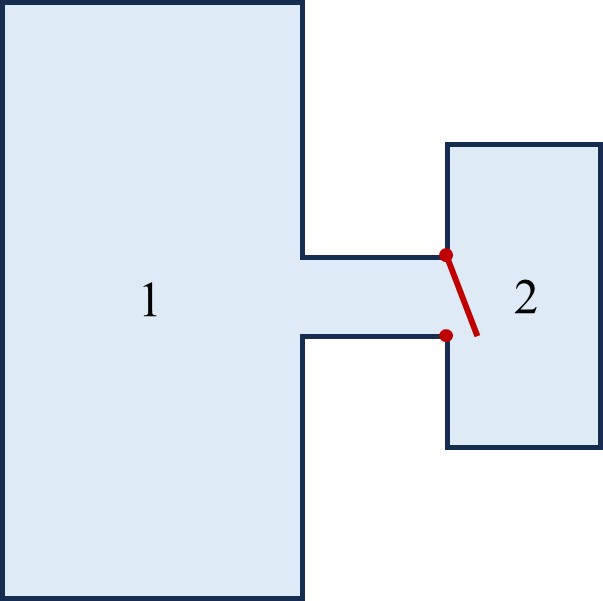
\includegraphics[width=0.25\linewidth]{../figs/VN12-Y24-PH-SYL-013P-3}
\end{center}
\begin{mcq}(4)
	\item $\SI{528}{\pascal/\kelvin}$.
	\item $\SI{521}{\pascal/\kelvin}$.
	\item $\SI{428}{\pascal/\kelvin}$.
	\item $\SI{421}{\pascal/\kelvin}$.
\end{mcq}
\hideall{
\textbf{Đáp án D.}\\
\begin{itemize}
	\item Xét quá trình nung từ $T_0$ đến $T_1$, khi van mở thì áp suất khí ở bình 1 là $\SI{E5}{\pascal}$:
	\begin{center}
		\begin{tabular}{C{4cm} C{3cm} C{4cm}}
			\colorbox{yellow}{\textcolor{red}{\textbf{Trạng thái 0}}} & $\xrightarrow[ ]{V=\text{const}}$ & \colorbox{yellow}{\textcolor{red}{\textbf{Trạng thái 1}}}\\
			$p_0=\SI{0.9E5}{\pascal}$ & &$p_1=\SI{E5}{\pascal}$\\
			$T_0=\SI{300}{\kelvin}$ & & $T_1=?$
		\end{tabular}
	\end{center}
$$\dfrac{p_0}{T_0}=\dfrac{p_1}{T_1}\Rightarrow T_1=\xsi{\dfrac{1000}{3}}{\kelvin}.$$
\item Khi van mở, một phần khí từ bình 1 tràn sang bình 2, do đó áp suất bình 1 giảm và áp suất bình 2 tăng. Khi đó, van lại đóng. Tiếp tục đun nóng 2 ngăn thì van giữ cho áp suất hai ngăn luôn chênh lệch $\Delta p=\SI{E5}{\pascal}$.\\
Áp dụng phương trình Claperon - Mendenleev:
$$ n=\dfrac{pV}{RT}\xrightarrow{ n= n_1+ n_2}\dfrac{p_0V_0}{T_0}=\dfrac{pV_1}{T}+\dfrac{\left(p-\SI{E5}{\pascal}\right)V_2}{T}\Rightarrow p=\SI{1.4E5}{\pascal}.$$
Vậy $\dfrac{p}{T_1}=\SI{420}{\pascal/\kelvin}.$
\end{itemize}
}


\end{enumerate}

\section{Trắc nghiệm đúng/sai}
\begin{enumerate}[label=\bfseries Câu \arabic*:, leftmargin=1.7cm]
	\item \mkstar{2}\\
	Một thùng có dung tích $\SI{20}{\liter}$ chứa $\SI{0.225}{\kilogram}$ khí helium tại nhiệt độ $\SI{18}{\celsius}$.
	\begin{enumerate}[label=\alph*)]
		\item Có $\SI{56.25}{\mole}$ khí helium trong thùng.
		\item Số phân tử khí helium trong thùng là $\SI{3.39E25}{}$.
		\item Áp suất trong thùng là $\SI{6.8E6}{\pascal}$.
		\item Áp suất trong thùng là $\SI{6.8}{atm}$.
	\end{enumerate}
\hideall{
\begin{enumerate}[label=\alph*)]
	\item Đúng.
	\item Đúng.
	\item Đúng.
	\item Sai. $p\approx\SI{67}{atm}$.
\end{enumerate}
}

\item\mkstar{3}\\
Một hỗn hợp không khí gồm $\SI{23.6}{\gram}$ khí oxygen và $\SI{76.4}{\gram}$ nitrogen ở áp suất $\SI{750}{\milli\meter Hg}$, nhiệt độ $\SI{27}{\celsius}$.
\begin{enumerate}[label=\alph*)]
	\item Thể tích hỗn hợp là $\SI{86.5}{\liter}$.
	\item  Khối lượng riêng của hỗn hợp là $\SI{1.16}{\gram/\liter}$.
	\item Áp suất riêng phần của oxygen là $\SI{160}{\milli\meter Hg}$.
	\item Áp suất riêng phần của nitrogen là $\SI{590}{\milli\meter Hg}$.
\end{enumerate}
\hideall{
\begin{enumerate}[label=\alph*)]
	\item Đúng.
	\item Đúng.
	\item Đúng.
	\item Đúng.
\end{enumerate}
}
	
	
	\item \mkstar{3}\\
	Trong ô tô, người ta thường đặt ở hệ thống tay lái một thiết bị nhằm bảo vệ người lái xe khi xe gặp tai nạn, gọi là túi khí. Túi khí được chế tạo bằng vật liệu co giãn tốt, chịu được áp suất lớn. Trong túi khí thường chứa $\ce{NaN_3}$, khi xe va chạm mạnh vào vật cản thì hệ thống cảm biến của xe sẽ kích thích chất rắn này làm nó phân huỷ tạo thành $\ce{Na}$ và khí $\ce{N_2}$. Do $\ce{Na}$ là kim loại hoạt động mạnh và có khả năng nổ nên người ta sử dụng $\ce{KNO_3}$ và $\ce{SiO_2}$ như là chất để ngăn cản sự gây hại của $\ce{Na}$. Toàn bộ quá trình phản ứng trong túi khí để tạo khí $\ce{N_2}$ làm căng đầy túi diễn ra một cách rất nhanh và có thể mô tả bằng 3 giai đoạn sau:
	\begin{enumerate}[label=\arabic*)]
		\item $\ce{NaN_3}\xrightarrow{} \ce{Na}+\dfrac{3}{2}\ce{N_2}$
		\item $2\ce{Na}+2\ce{KNO_3}\xrightarrow{}\ce{K_2O}+\ce{Na_2O}+2\ce{O_2}+\ce{N_2}$
		\item $\ce{K_2O}+\ce{SiO_2}\xrightarrow{}\ce{K_2SiO_3}.\ce{Na_2O}+\ce{SiO_2}\xrightarrow{}\ce{Na_2SiO_3}$
	\end{enumerate}
Biết trong túi khí có chứa $\SI{130}{\gram}$ chất rắn $\ce{NaN_3}$ và thể tích túi khí khi phồng lên có thể lên tới $\SI{48}{\liter}$, nhiệt độ $\SI{30}{\celsius}$. Để đơn giản cho việc tính toán, ta bỏ qua thể tích khí có trong túi trước khi phồng lên và thể tích các sản phẩm rắn được tạo thành trong phản ứng.
\begin{center}
	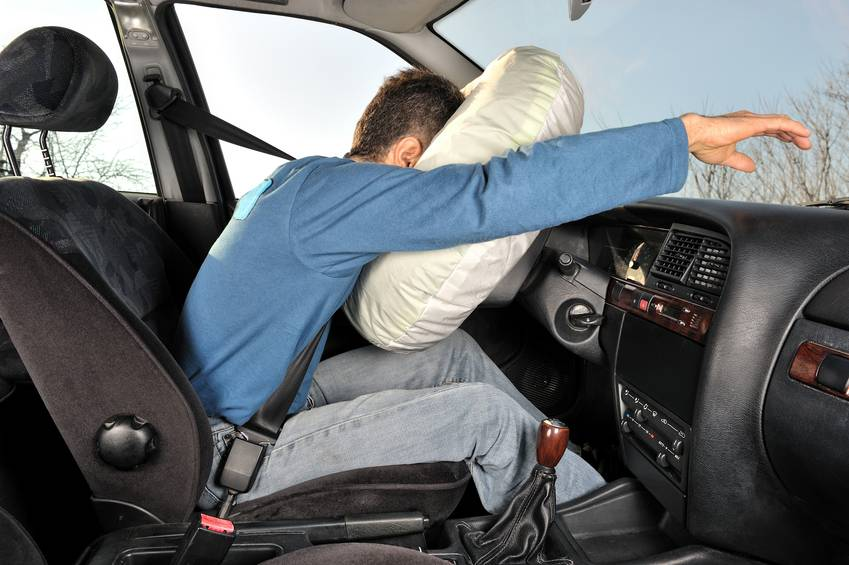
\includegraphics[width=0.35\linewidth]{../figs/VN12-Y24-PH-SYL-013P-2}
\end{center}
\begin{enumerate}[label=\alph*)]
	\item Số mol khí nitrogen được tạo thành trong túi khí là $\SI{3}{\mole}$.
	\item Áp suất khí trong túi sau phản ứng là $\SI{2.098E5}{\pascal}$.
	\item Khi va chạm với túi khí, thân người ép túi khí và làm giảm thể tích của nó đi $\SI{18}{\liter}$. Áp suất khí bên trong túi khi đó là $\SI{5.59e5}{\pascal}$.
	\item Nếu diện tích tiếp xúc giữa người và túi khi va chạm là $\SI{0.75}{\meter^2}$ thì phản lực do túi tác dụng lên người khi va chạm là xấp xỉ $\SI{252}{\kilo\newton}$.
\end{enumerate}
\hideall{
\begin{enumerate}[label=\alph*)]
	\item Sai. Số mole khí $\ce{N_2}$ tạo thành $ n_{\ce{N_2}}=2 n_{\ce{NaN_3}}=\SI{4}{\mole}.$
	\item Đúng.\\
	$$p=\dfrac{ n_{\ce{N_2}}RT}{V}=\SI{2.098E5}{\pascal}$$.
	\item Sai.
$$p'=\dfrac{pV}{V'}=\SI{3.36}{\pascal}.$$
\item Đúng.
\end{enumerate}
}
\end{enumerate}
\section{Bài tập tự luận}
\begin{enumerate}[label=\bfseries Câu \arabic*:, leftmargin=1.7cm]
	\item\mkstar{2}\\
	Một bình có dung tích $\SI{2}{\liter}$ chứa khí ở nhiệt độ $\SI{27}{\celsius}$ và áp suất $\SI{800}{\milli\meter Hg}$. Xác định số phân tử khí chứa trong bình. Cho biết trọng lượng riêng của thuỷ ngân $d=\SI{136E3}{\newton/\meter^3}$, số Avogadro $N_A=\SI{6.02E23}{\mole^{-1}}$.
	\hideall{
	Áp dụng phương trình Claperon - Mendeleev:
	$$pV=\dfrac{N}{N_A}RT\Rightarrow N=\dfrac{pVN_A}{RT}=\dfrac{\left(\SI{800E-3}{\meter}\right)\cdot\left(\SI{136E3}{\newton/\meter^3}\right)\cdot\left(\SI{2E-3}{\meter^3}\right)\cdot\left(\SI{6.02E23}{\mole^{-1}}\right)}{\left(\SI{8.31}{\joule/\mole\cdot\kelvin}\right)\cdot\left(\SI{300}{\kelvin}\right)}=\SI{5.25E22}{}.$$
}

\item \mkstar{2}\\
Tăng đồng thời nhiệt độ và áp suất của một khối khí lí tưởng từ $\SI{27}{\celsius}$ lên $\SI{177}{\celsius}$ và từ $\SI{100}{\kilo\pascal}$ lên $\SI{300}{\kilo\pascal}$. Khi đó, khối lượng riêng của khối khí tăng hay giảm bao nhiêu lần?
\hideall{
$$pV=\dfrac{m}{ M}RT\Rightarrow \rho=\dfrac{m}{V}=\dfrac{p M}{RT}$$
Khi thay đổi nhiệt độ và áp suất khối khí:
$$\dfrac{\rho_2}{\rho_1}=\dfrac{p_2}{p_1}\cdot\dfrac{T_1}{T_2}=2.$$
}

\item \mkstar{3}\\
{Một bình kín chứa một lượng khí có khối lượng $m=\SI{1.00}
	{\kilogram}$ ở áp suất $p_1=\SI{E7}{\pascal}$. Lấy ở bình ra một lượng khí cho tới khi áp suất khí còn lại trong bình là  $p_2=\SI{2.5E6}{\pascal}$. Tính khối lượng khí được lấy ra khỏi bình, biết nhiệt độ khí không đổi.
}
\hideall{Lượng khí trong bài tập này có khối lượng đã biết và thay đổi khi chuyển trạng thái.\\
	Trong quá trình chuyển trạng thái có hai thông số không đổi là thể tích $V$ và nhiệt độ $T$.
	\begin{center}
		\begin{tabular}{C{4cm} C{1.5cm} C{5cm}}
			\colorbox{green!40!white}{\textcolor{red}{\textbf{Trạng thái 1}}} & $\xrightarrow[]{V=const}$ & \colorbox{green!40!white}{\textcolor{red}{\textbf{Trạng thái 2}}}\\
			$m$ &&$m-\Delta m$\\
			$V_1=V$ & & $V_2=V$\\
			$T_1=T$ & & $T_2=T$\\
			$p_1=\SI{E7}{\pascal}$ & & $p_2=\SI{2.5E6}{\pascal}$
		\end{tabular}
	\end{center}
	Phương trình trạng thái của hai khí lí tưởng trên:
	\begin{equation*}
		\begin{cases}
			p_1V_1=\dfrac{m_1}{M}RT_1\Leftrightarrow p_1V=\dfrac{m}{M}RT\\
			p_2V_2=\dfrac{m_2}{M}RT_2\Leftrightarrow p_2V=\dfrac{\left(m-\Delta m\right)}{M}RT
		\end{cases}
	\end{equation*}
	\begin{eqnarray*}
		&\Rightarrow& \dfrac{m-\Delta m}{m}=\dfrac{p_2}{p_1}\\
		&\Rightarrow&\Delta m=m\cdot\left(1-\dfrac{p_2}{p_1}\right)=\left(\SI{1}{\kilogram}\right)\cdot\left(1-\dfrac{\SI{2.5E6}{\pascal}}{\SI{E7}{\pascal}}\right)=\SI{0.75}{\kilogram}.
	\end{eqnarray*}
}

\item \mkstar{3}\\
Trong bình chứa $\SI{10}{\liter}$ có chứa $\SI{4}{\mole}$ khí helium và $\SI{1.1}{\mole}$ khí oxygen. Nhiệt độ của khí trong bình là $\SI{295}{\kelvin}$. Tổng áp suất khí bên trong bình là bao nhiêu?
\hideall{
Tổng số mole khí:
$$n=n_{\ce{He}}+n_{\ce{O_2}}=\SI{5.1}{\mole}.$$
Tổng áp suất khí bên trong bình:
$$p=\dfrac{nRT}{V}\approx\SI{1.25}{\mega\pascal}.$$
}

\item \mkstar{3}\\
Một bình thể tích $V=\SI{20}{\liter}$ chứa một hỗn hợp khí hydrogen và helium ở nhiệt độ $t=\SI{20}{\celsius}$, áp suất $\SI{200}{\kilo\pascal}$. Khối lượng của hỗn hợp  khí là $m=\SI{5.00}{\gram}$. Tìm khối lượng của mỗi chất khí trong hỗn hợp.
\hideall{
\begin{equation}
	\label{eq:13P-7}
	m_{\ce{H_2}}+m_{\ce{He}}=\SI{5}{\gram}
\end{equation}
Phương trình Claperon - Mendeleev:
\begin{equation}
	\label{eq:13P-8}
	pV=\left(\dfrac{m_{\ce{H_2}}}{ M_{\ce{H_2}}}+\dfrac{m_{\ce{He}}}{ M_{\ce{He}}}\right)RT\Rightarrow \dfrac{m_{\ce{H_2}}}{ M_{\ce{H_2}}}+\dfrac{m_{\ce{He}}}{ M_{\ce{He}}}\approx1,642
\end{equation}
Từ (\ref{eq:13P-7}) và (\ref{eq:13P-8}) suy ra:
$$\begin{cases}
	m_{\ce{H_2}}=\SI{1.568}{\gram}\\
	m_{\ce{He}}=\SI{3.432}{\gram}
\end{cases}.$$
}

\item \mkstar{3}\\
Làm thí nghiệm người ta thấy bình chứa $\SI{1}{\kilogram}$ khí nitrogen bị nổ ở nhiệt độ $\SI{350}{\celsius}$. Tính khối lượng khí hydrogen có thể chứa trong bình cùng loại ở nhiệt độ $\SI{50}{\celsius}$ và hệ số an toàn là 5, nghĩa là áp suất tối đa chỉ bằng $1/5$ áp suất gây nổ.
\hideall{
Áp dụng phương trình Claperon - Mendeleev:
$$pV=\dfrac{m}{ M}RT\Rightarrow \dfrac{p_{\ce{H_2}}}{p_{\ce{N_2}}}=\dfrac{m_{\ce{H_2}}}{m_{\ce{N_2}}}\cdot \dfrac{ M_{\ce{N_2}}}{ M_{\ce{H_2}}}\cdot\dfrac{T_{\ce{H_2}}}{T_{\ce{N_2}}}\Rightarrow m_{\ce{H_2}}=\SI{27.55}{\gram}.$$
}

\item \mkstar{3}\\
Một bình cầu thuỷ tinh được cân 3 lần trong các điều kiện:
\begin{enumerate}[label=\alph*)]
	\item đã hút chân không;
	\item chứa đầy không khí ở điều kiện tiêu chuẩn;
	\item chứa đầy một lượng khí nào đó ở áp suất $p=\SI{1.5}{atm}$.
\end{enumerate}
Khối lượng tương ứng trong từng lần cân là $m_1=\SI{200}{\gram}$; $m_2=\SI{204}{\gram}$; $m_3=\SI{210}{\gram}$.
Nhiệt độ coi như không đổi. Khối lượng mole của khí trong lần cân thứ ba bằng bao nhiêu?
\hideall{
Khối lượng không khí trong lần cân thứ 2 là: $m_\text{k2}=m_2-m_1=\SI{4}{\gram}$.\\
Khối lượng khí trong lần cân thứ 3 là: $m_\text{k3}=m_3-m_1=\SI{10}{\gram}$.\\
Áp dụng phương trình Claperon - Mendeleev:
$$pV=\dfrac{m}{ M}RT\Rightarrow \dfrac{p_3}{p_2}=\dfrac{m_\text{k3}}{m_\text{k2}}\cdot\dfrac{ M_\text{k2}}{ M_\text{k3}}\Rightarrow  M_\text{k3}\approx\SI{48.3}{\gram/\mole}.$$
}

\item \mkstar{3}\\
Một bình chứa $\SI{0.3}{\kilogram}$ khí helium. Sau một thời gian, do bị hở, khí bị thoát ra một phần. Biết rằng, nhiệt độ tuyệt đối của khí giảm $\SI{10}{\percent}$, áp suất giảm $\SI{20}{\percent}$. Số nguyên tử khí đã thoát khỏi bình là bao nhiêu?
\hideall{
Áp dụng phương trình Claperon - Mendeleev:
$$pV=\dfrac{m}{ M}RT\Rightarrow \dfrac{p_2}{p_1}=\dfrac{m_2}{m_1}\cdot\dfrac{T_2}{T_1}\Rightarrow m_2=\xsi{\dfrac{4}{15}}{\kilogram}.$$
Số nguyên tử khí thoát ra:
$$N=\dfrac{\left(m_1-m_2\right)}{ M}\cdot N_A\approx\SI{5E24}{}.$$
}

\item \mkstar{3}\\
Trong cylanh kín, ở giữa đặt một piston dẫn nhiệt và có thể chuyển động không ma sát. Bên trái cylanh chứa $\SI{1}{\kilogram}$ khí carbon dioxide, còn bên phải chứa $\SI{1}{\kilogram}$ khí hydrogen. Hãy xác định tỉ số thể tích của khí carbon dioxide và khí hydrogen khi cân bằng (cân bằng nhiệt và cân bằng cơ học).
\begin{center}
	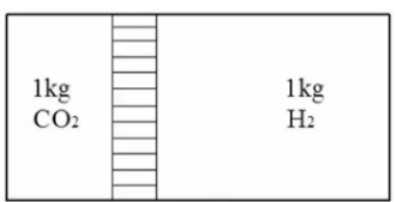
\includegraphics[width=0.35\linewidth]{../figs/VN12-Y24-PH-SYL-013P-1}
\end{center}
\hideall{
$$pV=\dfrac{m}{ M}RT\xrightarrow[p_{\ce{H_2}}=p_{\ce{CO_2}}]{T_{\ce{H_2}}=T_{\ce{CO_2}}}\dfrac{V_{\ce{H_2}}}{V_{\ce{CO_2}}}=\dfrac{ M_{\ce{CO_2}}}{ M_{\ce{H_2}}}=\dfrac{44}{2}=22.$$
}

\item \mkstar{3}\\
Hai bóng đèn thuỷ tinh giống hệt nhau được nối với nhau bằng một ống thuỷ tinh mỏng. Khí được nạp  vào các bóng đèn này tại điều kiện tiêu chuẩn. Nếu đặt một bóng đèn thuỷ tinh vào nước đá và bóng còn lại vào nước nóng thì áp suất khí tăng gấp 1,5 lần. Xác định nhiệt độ của nước nóng.
\begin{center}
	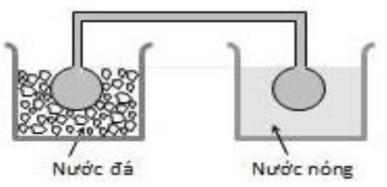
\includegraphics[width=0.35\linewidth]{../figs/VN12-Y24-PH-SYL-013P-4}
\end{center}
\hideall{
\begin{center}
	\begin{tabular}{|L{3cm}|C{3cm}|C{3cm}|C{3cm}|}
		\hline
		&$p$& $V$&$T$\\
		\hline
		Ban đầu & $p_0$ & $2V$ & $\SI{273}{\kelvin}$\\
		\hline
		Nước đá & $1,5p_0$ & $V$ & $\SI{273}{\kelvin}$\\
		\hline
		Nước nóng & $1,5p_0$ & $V$ &  $T$\\
		\hline
	\end{tabular}
\end{center}
$$ n=\dfrac{pV}{RT}\xrightarrow{ n= n_1+ n_2}\dfrac{p_0\cdot2V}{R\cdot273}=\dfrac{1,5p_0\cdot V}{273R}+\dfrac{1,5p_0\cdot V}{R\cdot T_2}\Rightarrow T_2=\SI{819}{\kelvin}\Rightarrow t_2=\SI{546}{\celsius}.$$
}
\end{enumerate}






